\subsection*{JGAP}
To implement the operators and benchmarks described earlier, we have built upon the JGAP framework. JGAP is an open source Genetic Algorithms package for the Java programming language developed by Meffert et al \cite{jgap}. This work is built upon JGAP version 3.6.2, which was the latest stable release at the time this paper was written.

\subsection*{Experimentation Setup}

To determine how well any Genetic Algorithm performs, it is important to know which of the many available operators and configurations were utilized. The same setup was used for each experiment measuring solution quality, and is outlined in Figure \ref{fig:GA-config}. These parameters are similar to those found in the literature to ensure that our results are comparable to previous research \cite{Sudholt12, Eiben95, Eiben96}. 

\begin{figure}[h]
\begin{center}
\begin{tabular}{ | l | c | }
\hline
parents used for recombination & 2-10, by steps of 2 \\
\hline
selection type & steady-state \\
\hline
selection mechanic & best first \\
\hline
diagonal crossover rate & 70 \% \\
\hline
fitness-based scanning rate & 70 \% \\
\hline
elitist schema overlay rate & 100 \% \\
\hline
mutation rate & dynamic \cite{Back93} \\
\hline
population size & fixed at 200 \\
\hline
termination condition & 500 generations elapsed \\
\hline
trials per configuration & 100 \\
\hline
\end{tabular}
\caption{Parameters used for testing}
\label{fig:GA-config}
\end{center}
\end{figure}

All of our experiments measuring runtime were executed on an Intel Core i5-2500 processor clocked at 3.30 gigahertz to ensure that the data gathered was comparable. The computer also had 16 gigabytes of RAM and was running version 5.5 of the CentOS operating system. 

\subsubsection*{Benchmark Parameters}
To ensure that our tests are reproducible, the parameters used to generate each of our test cases have also been included. The n-dimensional numerical optimization problems were tested on genetic sequences of length $100$, split into $4$ dimensions of $25$ boolean alleles: For reference, they have been listed below:

\begin{itemize}
\item De Jong's Hypersphere Function
\item De Jong's Hyper-ellipsoid Function
\item The Sum of Powers Function
\item Griewank's Function
\item Rastrigin's Function
\item Rosenbrock's Function
\end{itemize} 

The 2-dimensional functions were tested on genetic sequences of length $62$, with the boolean alleles split evenly between the two dimensions. They have also been listed below:

\begin{itemize}
\item Michaelwicz's Function
\item The Six-Hump Camel Back Function
\item Schubert's Function
\end{itemize}

Both the Knapsack and the Traveling Salesman problems were tested on several randomly generated instances of size $50$ to $500$ by increments of $50$. $10$ instances of each size were generated to help prevent against a particular operator having an advantage over another due to its ability to exploit a feature of a given instance. NK-Landscapes were similarly generated for $n = 50$ to $n = 250$ with increments of $50$. $20$ instances were generated for each size, $10$ with $k = 5$ and the remainder with $k = 10$. Both NK-Landscapes and Knapsack Problem instances were tested using boolean alleles, and the Traveling Salesman Problem used integer alleles.

\subsection*{Results}
To determine the usefulness of elitist schema overlays as a genetic operator, we compared our work to current successful operators. To do so, we have analyzed both how efficient our operator is and how well it contributes to solution quality. 

The efficiency data is drawn from runtimes while minimizing instances of increasing size of the first De Jong function over $150$ generations. A numerical optimization function was chosen to limit error stemming from variance in the time required to read the input files that stored instances of NP-Hard problems. De Jong's Hypersphere function was specifically selected since the population converged to the optimal solution in each of our experiments. This allowed us to account for variance in the time necessary to construct elitist schema overlays with respect to the similarity of high performing genetic sequences.

To measure solution quality for each operator, we measured the average fitness of the most fit solution found for each of the numerical optimization problems. To measure the solution quality of problems in NP-Hard, we measured the frequency at which each operator found the best known solution across the problems all operators. It should be noted that the best found solutions during experimentation for $k$-value selection were only compared against other methodologies in that section; the best found solutions during experiments comparing elitist schema overlays to multi-parent operators were drawn from across both of these datasets. We tested several instances of each size of each problem to reduce error, and collected frequency data to allow us to compare solutions of different instances that were the same size. Multiple instances were used because internal features of a given instance may play a role in how well a particular operator performs. All of this data was used to help answer the following questions:

\begin{itemize}
\item Do fitness-based scanning and diagonal crossover perform as previously reported, with more parents tending to higher success rates?
\item Do fitness-based scanning and diagonal crossover perform better when used separately or in conjunction with each other? 
\item Which of the three methods of selecting $k$, assigning random values, selecting a fixed percentage, or by computing a linear relationship with generations left, performs best?
\item How do each of the above methods of $k$ selection affect the convergence rates of their respective populations?
\item With which genetic operator(s) does the best performing elitist schema overlay configuration perform best?
\item Do elitist schema overlays improve solution quality?
\item How efficiently can elitist schema overlays be computed and applied in relation to other genetic operators?
\end{itemize}

To answer these questions, we will first explore the genetic operators from the literature. Secondly, we compare the various methodologies used to select a $k$-value for elitist schema overlays to determine which we will test in conjunction with existing genetic operators. Finally, we will analyze how elitist schema overlays perform when used in conjunction with existing genetic operators.

\subsubsection*{Existing Genetic Operators}
To determine if elitist schema overlays improve the overall performance of Genetic Algorithms, we must first establish a performance baseline from the existing research. To do so, we have tested both diagonal crossover and fitness-based scanning individually and in conjunction with each other against our benchmarks. Diagonal crossover and fitness-based scanning were both tested with arities of 2, 4, 6, 8, and 10. When combined, both operators were set to the same arity from the previous list. 

\begin{figure}[htbp!]
\centering
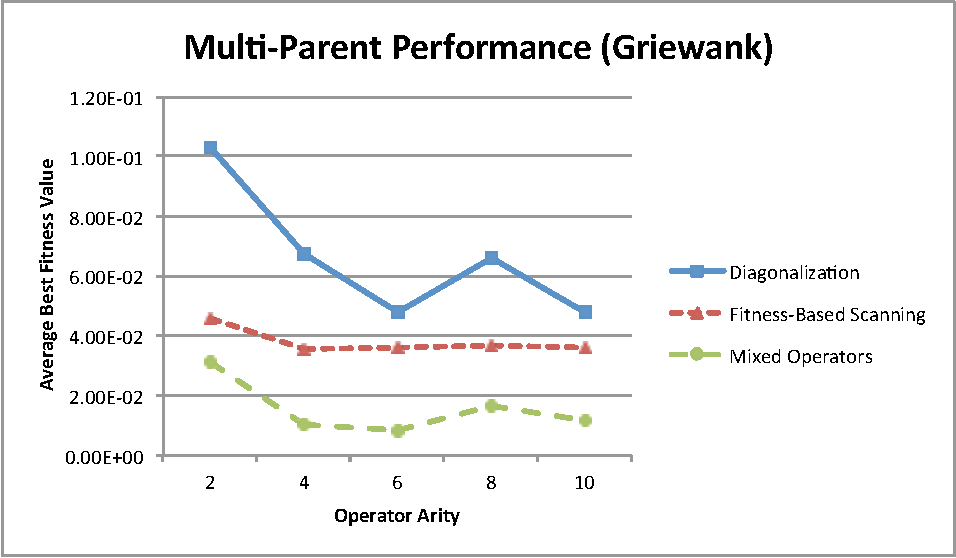
\includegraphics[scale=0.70]{charts/MP_Griewank.pdf}
\caption{Multi-Parent Performance on Griewank's Function}
\label{fig:mp_griewank}
\end{figure}

\begin{figure}[htbp!]
\centering
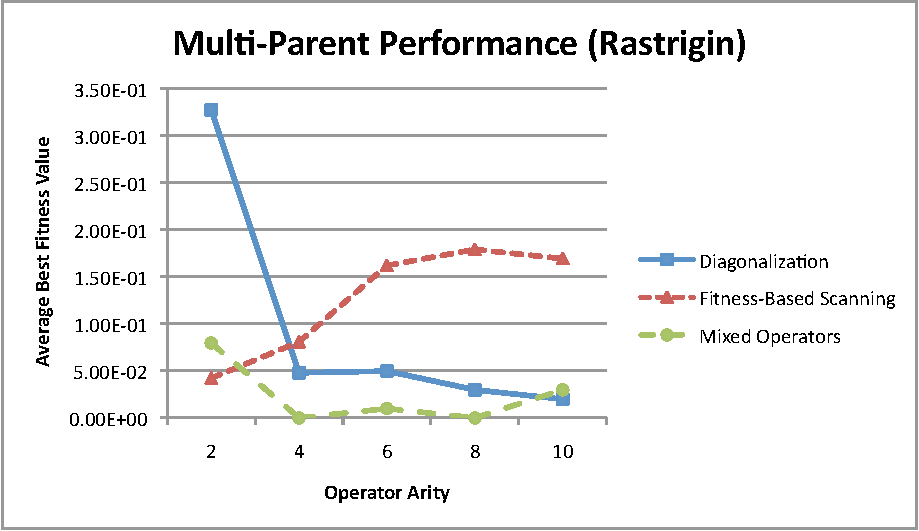
\includegraphics[scale=0.70]{charts/MP_Rastrigin.pdf}
\caption{Mulit-Parent Performance on Rastrigin's Function}
\label{fig:mp_rastrigin}
\end{figure}

\begin{figure}[htbp!]
\centering
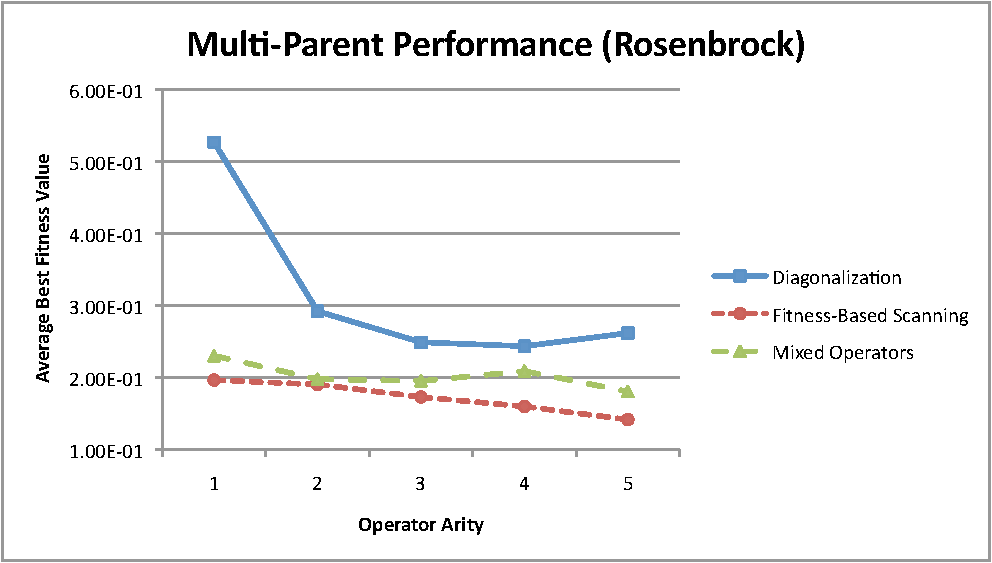
\includegraphics[scale=0.70]{charts/MP_Rosenbrock.pdf}
\caption{Multi-Parent Performance on Rosenbrock's Function}
\label{fig:mp_rosenbrock}
\end{figure}

Each of the operator configurations consistently found the same minima for 6 of the 9 optimization problems. Since this data does not differentiate the operators, we will focus upon the remaining three functions:  Griewank's (referenced in Figure \ref{fig:mp_griewank}), Rastrigin's (Figure \ref{fig:mp_rastrigin}), and Rosenbrock's (Figure \ref{fig:mp_rosenbrock}).

In these cases, traditional Genetic Algorithms consistently performed worse than multi-parent strategies. As a general trend, both utilizing more operators and increasing the arity of those operators increased performance, but there were exceptions. Fitness-based scanning saw performance degradation with arity 10 on the Rastrigin function, as did mixed operator usage on the Griewank function. Utilizing several operators performed the best on the Griewank and Rastrigin functions, and was outperformed on the Rosenbrock function by fitness-based scanning.

We also observed that diagonalization was consistently outperformed on both the Rosenbrock and Griewank functions; however, diagonalization did outperform fitness-based scanning on the Rastrigin function. Each of these findings were in line with the literature on fitness-based scanning and diagonalization \cite{Eiben94, Eiben95}. We will now investigate how these operators performed on the NP-Hard test problems.

\begin{figure}[htbp!]
\centering
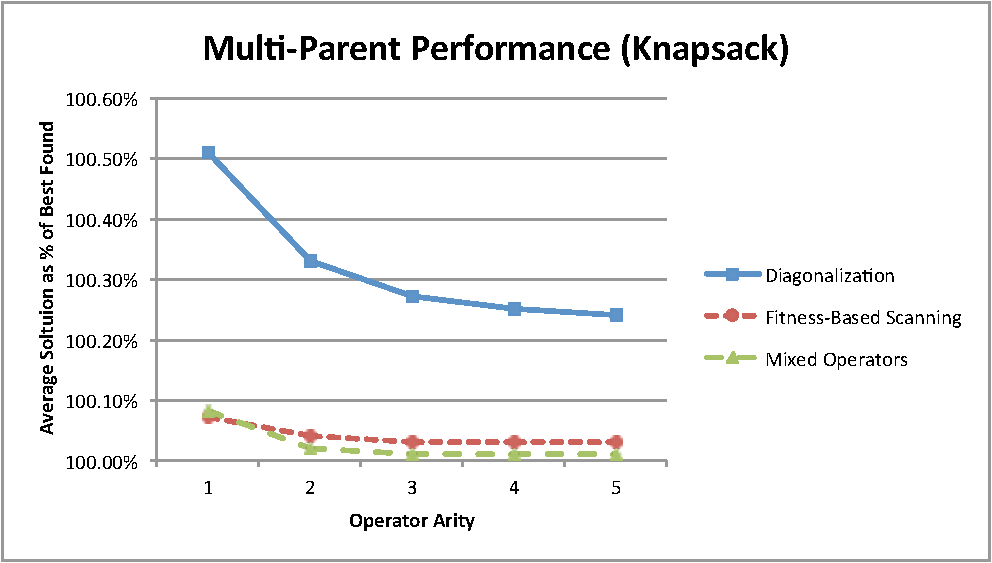
\includegraphics[scale=0.70]{charts/MP_Knapsack.pdf}
\caption{Multi-Parent Performance on the Knapsack Problem}
\label{fig:mp_knapsack}
\end{figure}

For the Knapsack Problem (referenced in Figure \ref{fig:mp_knapsack}), diagonalization consistently performs worse than all other configurations; however, in the worst case, the instances with 500 objects, its average best solution was only $1.39\%$ higher than the best found solution across all configurations, where the best strategy found solutions $0.01\%$ greater than the optimal when averaging over all instances of all sizes. Within that range of performance, our previous observation that increasing the arity of the operators improved performance held true.

\begin{figure}[htbp!]
\centering
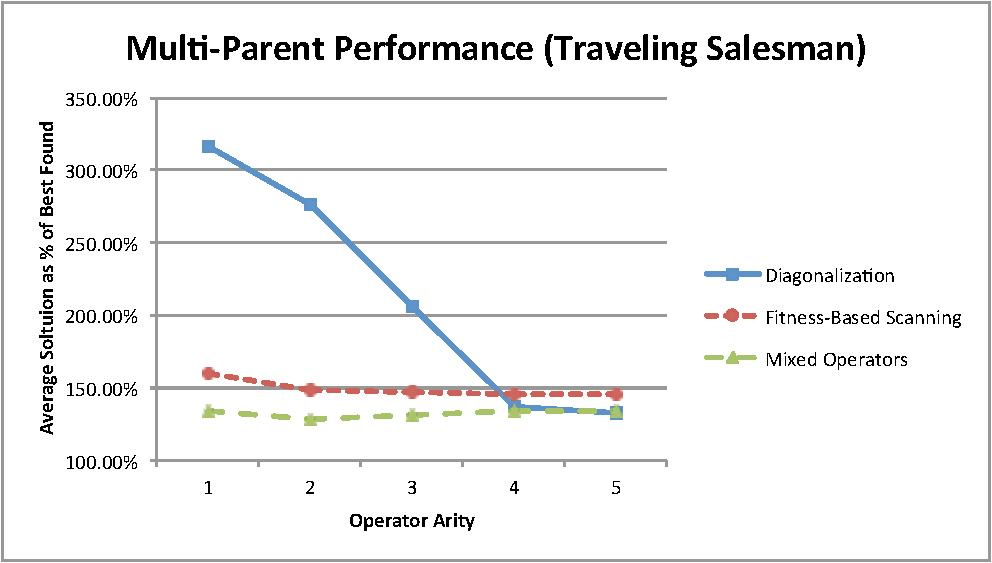
\includegraphics[scale=0.70]{charts/MP_TSP.pdf}
\caption{Multi-Parent Performance on the Traveling Salesman Problem}
\label{fig:mp_tsp}
\end{figure}

Within the tested instances of the Traveling Salesman Problem (referenced in Figure \ref{fig:mp_tsp}), high-arity diagonalization outperformed fitness-based scanning, but was outperformed by mixed operator strategies. Mixed operator strategies performed the best with arity 4, but across the other two strategies, more parents typically increased performance. Once again, traditional Genetic Algorithms performed the worst, and found solutions $216.52\%$ greater than the best found when averaged across all instances for all problem sizes, where the best averaged performance was $31.47\%$ greater than the best found on average.

As previously found, multi-parent strategies performed the best when tested on NK-Landscapes \cite{Eiben96}. For each problem instance, the best found solution was always found by each operator configuration.

Overall, this data supports previous conclusions about the success of genetic operators with arities greater than $2$. Increasing the number of parents involved in recombination improved the success of both diagonalization and fitness-based scanning. Additionally, utilizing both of these operators in conjunction with each-other further increased performance on both the numerical optimization and NP-Hard test problems. 

Now we will compare the various methodologies of $k$ selection with elitist schema overlays, and compare the best found strategy to the multi-parent operators tested here. 

\subsubsection*{$k$-Value Selection Methodologies}
Each of our $k$ selection methodologies was used in addition to a traditional Genetic Algorithm to determine which methodology performed the best. When using $k$ as a fixed percentage of the population, we ran tests with $k$ set to $10\%, 20\%, 30\%, 40\%, 50\%, 60\%, 70\%, 80\%,\text{and } 90\%$. During our tests with $k$ chosen as a linear relationship with the number of generations remaining, we determined $k$ with the following formula:
\[
k = \left\lfloor \frac{generationsLeft}{totalGenerations} * populationSize \right\rfloor
\]

As before, 6 of the 9 numerical optimization problems lead to each of the operators converging to the same solution. The solution quality information from these cases does not help us differentiate these operators, but the convergence information from these tests will be explored later. The remaining functions to be analyzed for solution quality information are the following: Griewank's (referenced in Figure \ref{fig:eso_griewank}), Rastrigin's (Figure \ref{fig:eso_rastrigin}), and Rosenbrock's (Figure \ref{fig:eso_rosenbrock}).

\begin{figure}[htbp!]
\centering
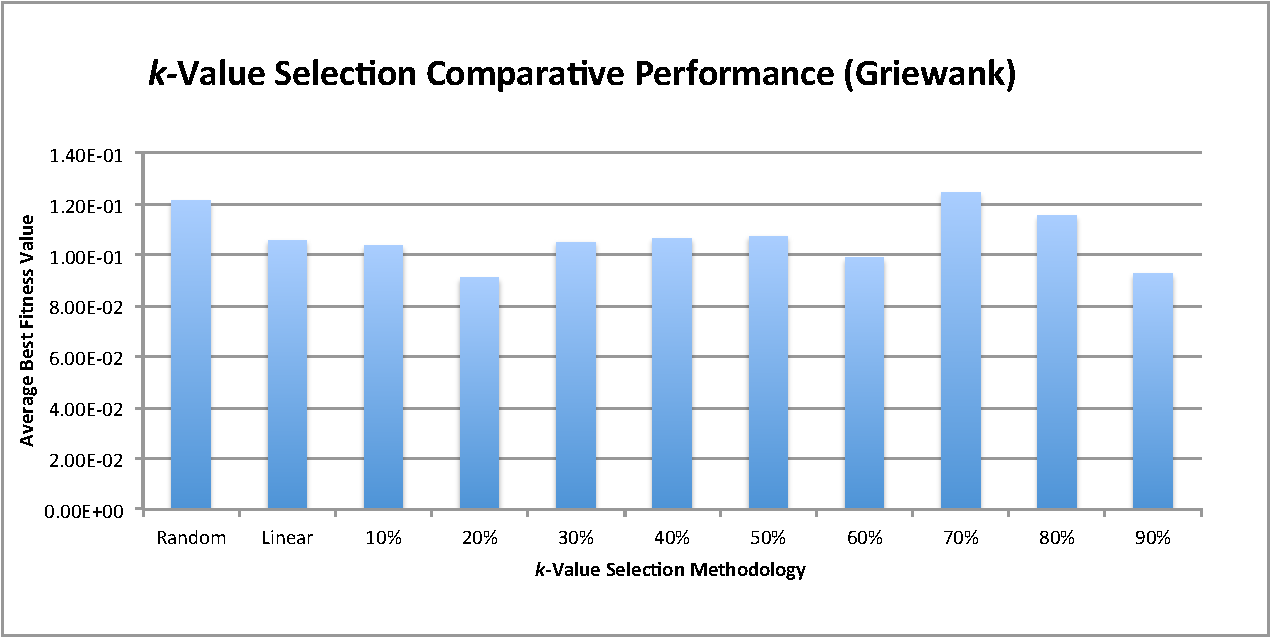
\includegraphics[scale=0.60]{charts/ESO_Griewank.pdf}
\caption{Elitist Schema Overlay Performance on Griewank's Function}
\label{fig:eso_griewank}
\end{figure}

\begin{figure}[htbp!]
\centering
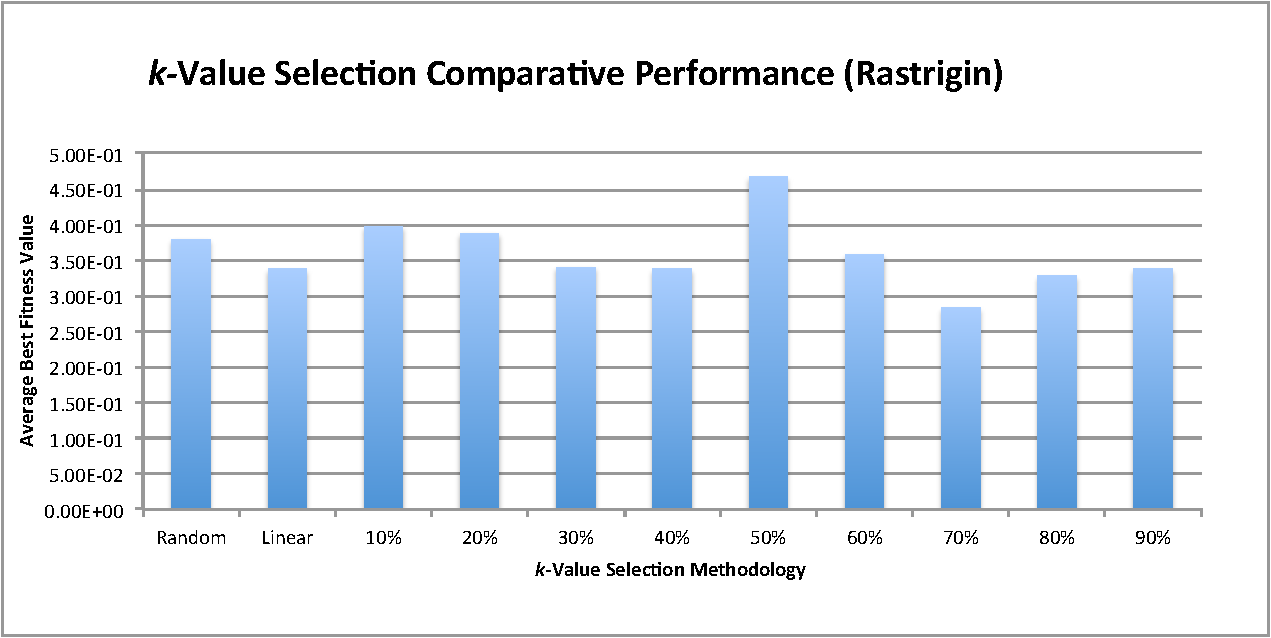
\includegraphics[scale=0.60]{charts/ESO_Rastrigin.pdf}
\caption{Elitist Schema Overlay Performance on Rastrigin's Function}
\label{fig:eso_rastrigin}
\end{figure}

\begin{figure}[htbp!]
\centering
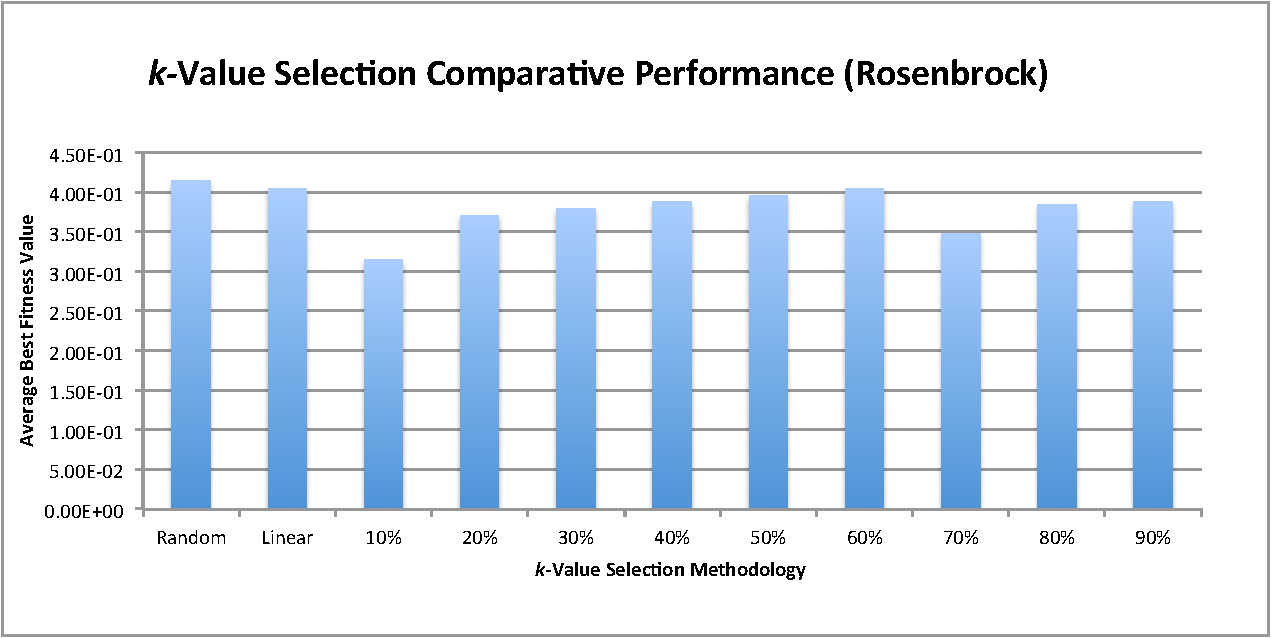
\includegraphics[scale=0.60]{charts/ESO_Rosenbrock.pdf}
\caption{Elitist Schema Overlay Performance on Rosenbrock's Function}
\label{fig:eso_rosenbrock}
\end{figure}

Across each of these functions, no single methodology consistently dominated the others. Further, when analyzing the data across the percentage based selection methods, the percent used and the overall performance did not appear to be correlated. Selecting $k$ randomly consistently converged the slowest, taking $153.28$ generations on average, and selecting $k = 30\%$, the fastest converging methodology, lead to convergence after $130.7$ generations on average. We will now investigate the behavior of traditional Genetic Algorithms with elitist schema overlays on problems in NP-Hard.

%
% ESO Knapsack Data goes here
%

The solution quality data gathered from the Knapsack Problem is almost indistinguishable, much like the numerical optimization data was. Every methodology found on average a solution that was between $100.19\%$ and $100.21\%$ of the best found solution for that given instance. The convergence data was more varied. Selecting $k = 20\%$ converged on average after $161.78$ generations, and $k = 40\%$ converged the fastest, taking $142.09$ generations on average. 

%
% ESO TSP Data goes here
%

%
% ESO NK Convergence Data goes here
%

As was the case with multi-parent Genetic Algorithms, our tests with elitist schema overlays on NK-Landscape instances gave us little data to differentiate methodologies. Following the trend of the other problems in NP-Hard, $k = 20\%$ converged the slowest, taking $33.97$ generations on average, and $k = 40\%$ converged the fastest, taking $22.48$ generations on average. 

\begin{figure}[htbp!]
\centering
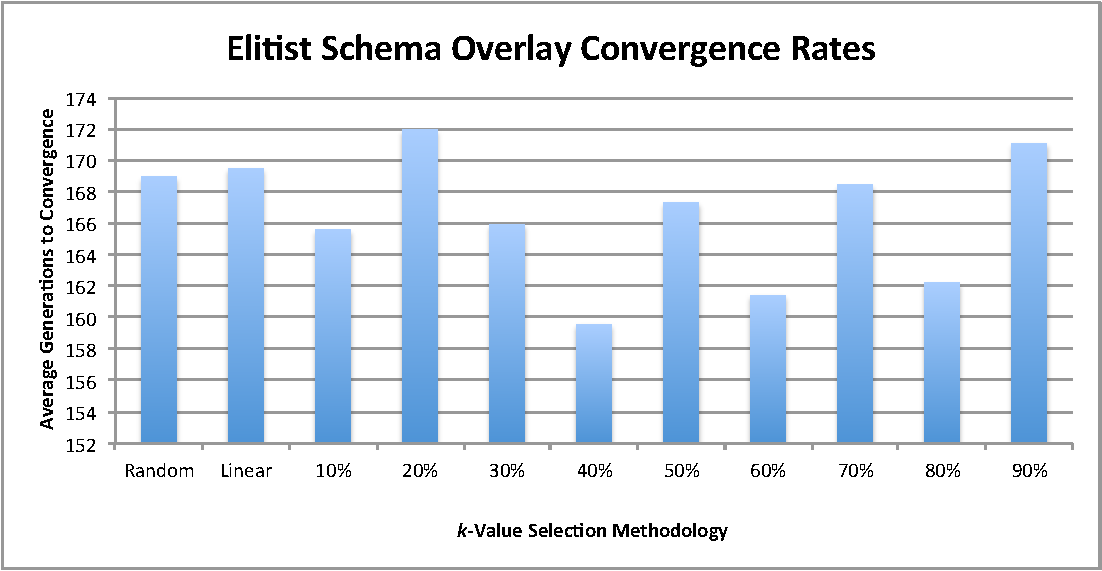
\includegraphics[scale=0.70]{charts/Convergence.pdf}
\caption{Elitist Schema Overlay Rates of Convergence}
\label{fig:eso_convergence}
\end{figure}

To gather generalized convergence rate data, we averaged the number of generations to convergence across all runs of all problem instances (Referenced in Figure \ref{fig:ESO-convergence}). There appears to be no correlation between the number of parents in fixed percentage methodologies and the average rate of convergence. As was the case before, $k=20\%$ converged the slowest on average while $k=40\%$ converged the quickest. This data helped us select a $k$-value selection methodology to utilize with both traditional Genetic Algorithms and multi-parent operators to determine empirically how they affect performance.

\subsubsection*{Elitist Schema Overlays with Existing Operators}
We chose to run our further experiments with $k$ set to be a fixed $20\%$ of our population. The rationale behind this choices was based upon the observed convergence rates in our experiments. Since most of the solutions were comparable in quality, we focused upon the methodology that converged the slowest. This decision was made in an attempt to help prevent premature convergence \cite{Andre01}. We also aimed to maintain the disruptiveness of diagonalization and fitness-based scanning, which is thought to be central to the successes of multi-parent operators \cite{Eiben95}. This was used in conjunction with the $15$ different genetic operator configurations used in the experiments with the existing genetic operators. We will begin by comparing performance on the numerical optimization functions.

\begin{figure}[htbp!]
\centering
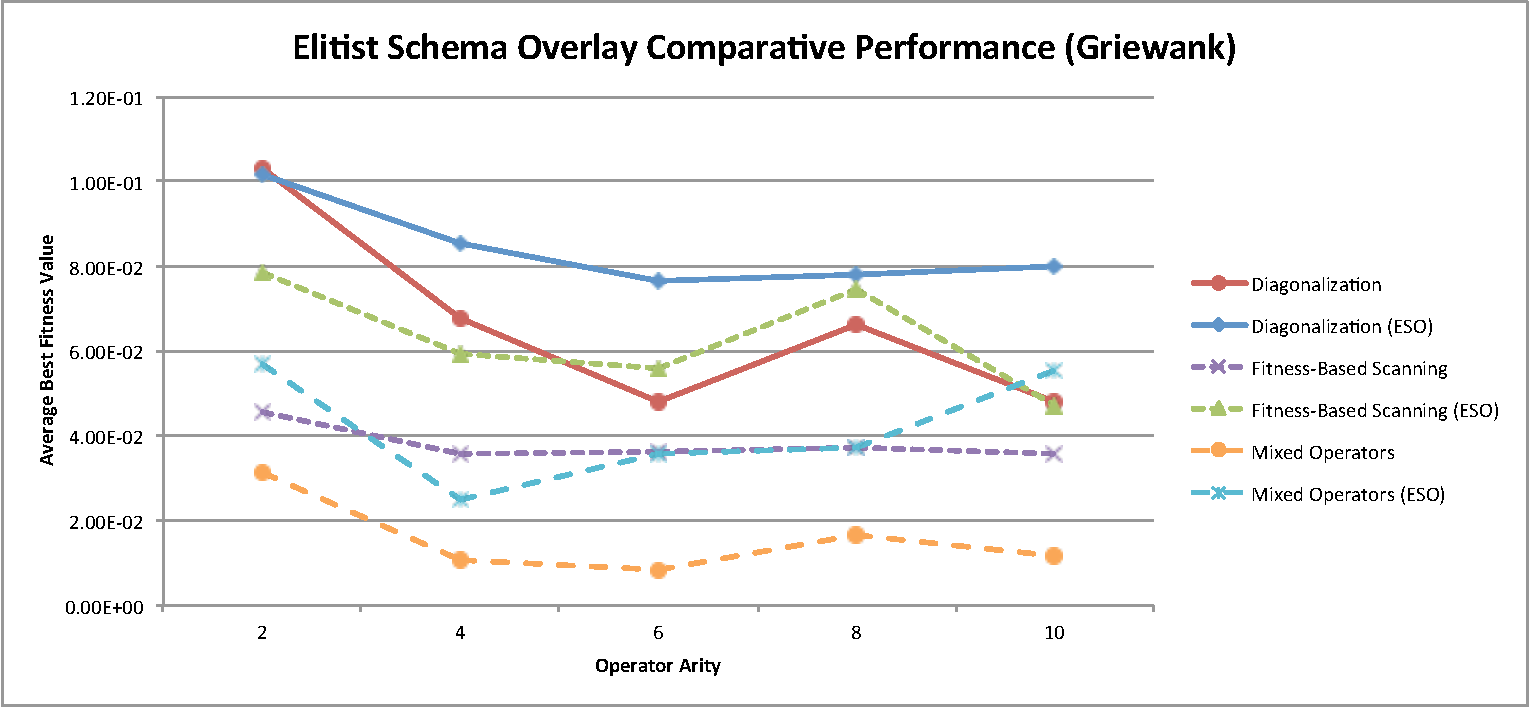
\includegraphics[scale=0.60]{charts/Both_Griewank.pdf}
\caption{Comparative Performance on Griewank's Function}
\label{fig:both_griewank}
\end{figure}

\begin{figure}[htbp!]
\centering
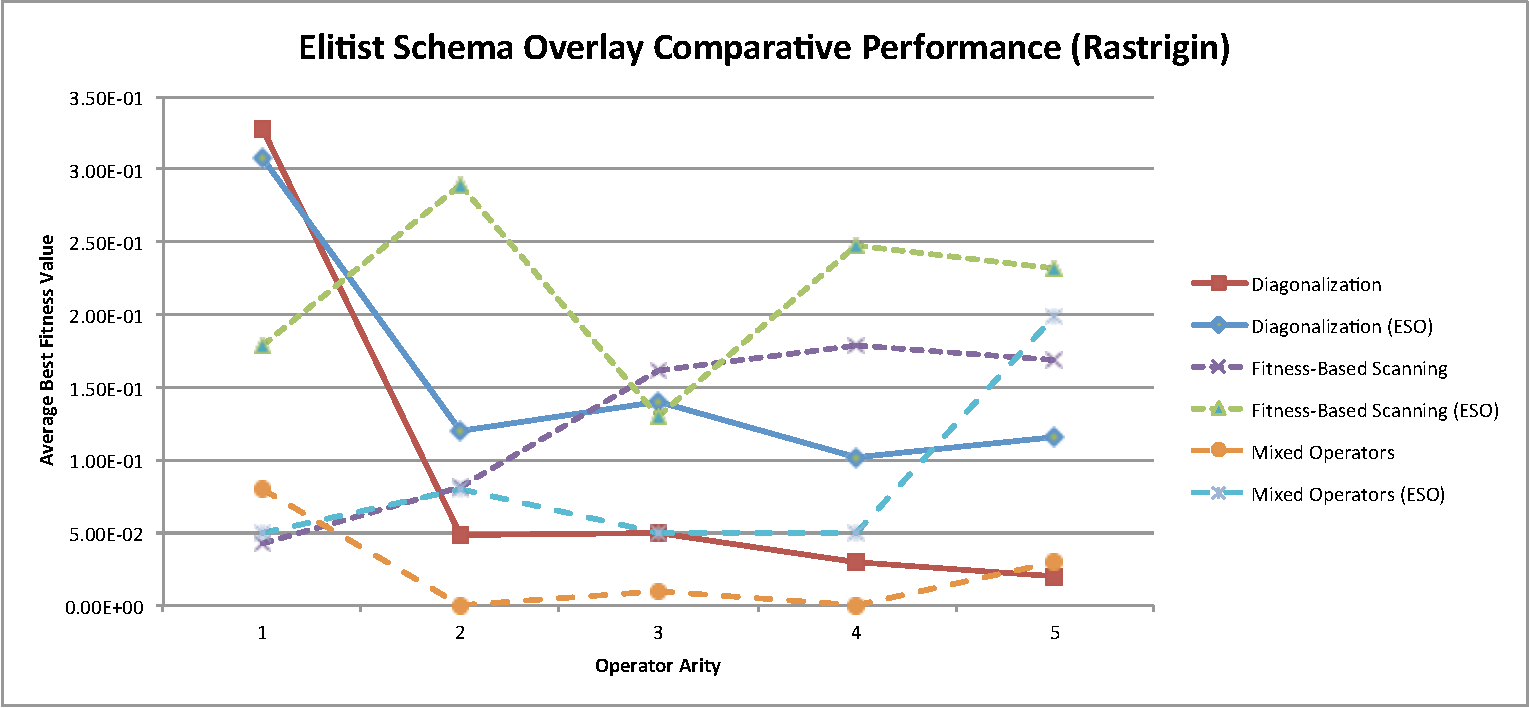
\includegraphics[scale=0.60]{charts/Both_Rastrigin.pdf}
\caption{Comparative Performance on Rastrigin's Function}
\label{fig:both_rastrigin}
\end{figure}

\begin{figure}[htbp!]
\centering
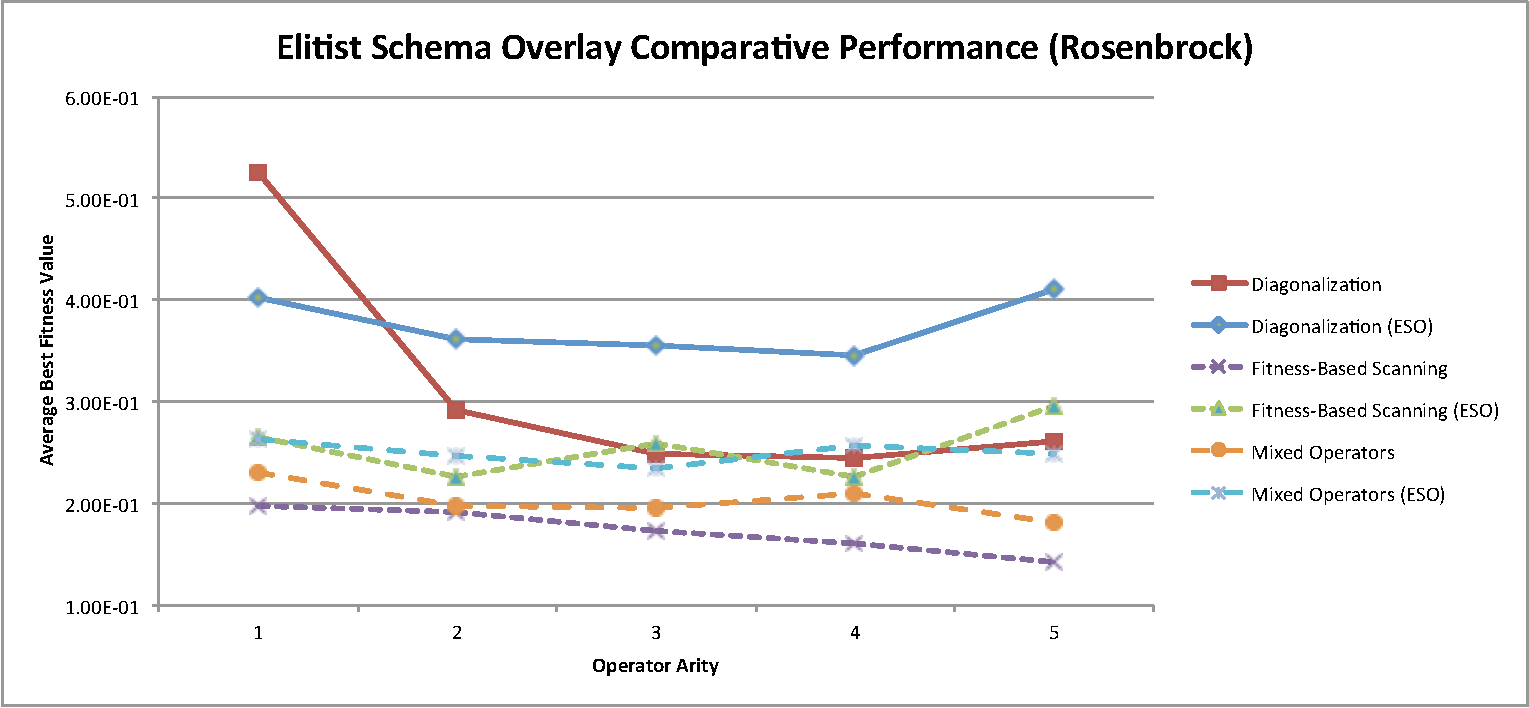
\includegraphics[scale=0.60]{charts/Both_Rosenbrock.pdf}
\caption{Comparative Performance on Rosenbrock's Function}
\label{fig:both_rosenbrock}
\end{figure}

As before, the observed performance on the numerical optimization problems only deviated during tests on Griewank's function (referenced in Figure \ref{fig:both_griewank}), Rastrigin's function (Figure \ref{fig:both_rastrigin}), and Rosenbrock's function (Figure \ref{fig:both_rosenbrock}). Across these tests, multi-parent operators without elitist schema overlays tend to outperform those with elitist schema overlays. The tests run with elitist schema overlays show similar relative behavior when compared to each other as the multi-parent operators without elitist schema overlays; that is, diagonalization was usually outperformed by fitness-based scanning, which was in turn out performed by a multiple-operator strategy. In contrast to the previous experiment, increasing the number of parents no longer resulted in improved performance in the average case.

\begin{figure}[htbp!]
\centering
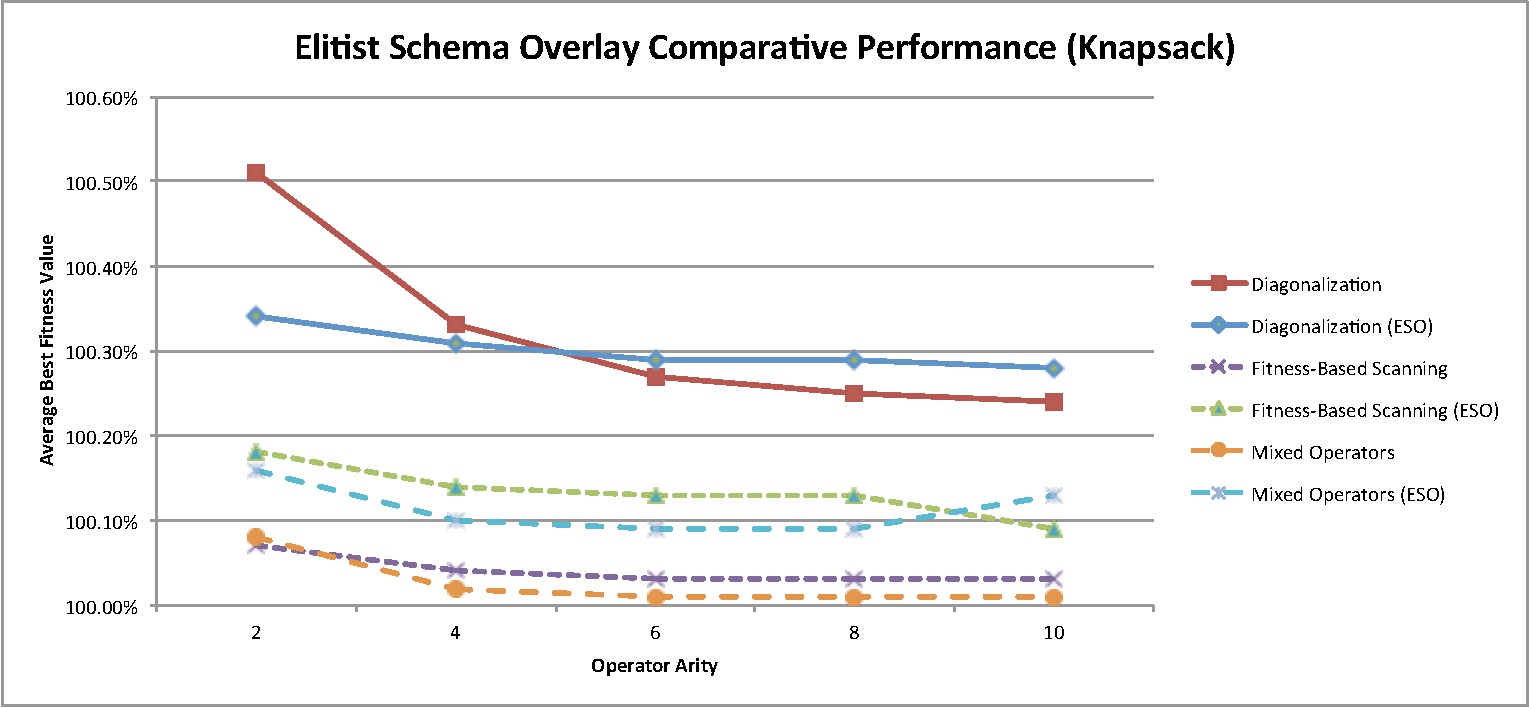
\includegraphics[scale=0.60]{charts/Both_Knapsack.pdf}
\caption{Comparative Performance on the Knapsack Problem}
\label{fig:both_knapsack}
\end{figure}

Within the data gathered for the Knapsack Problem (referenced in Figure \ref{fig:both_knapsack}), the use of elitist schema overlays decreased the average performance of all operators by an average $0.05$ percentage points; however, when utilized with traditional Genetic Algorithms, elitist schema overlays increased performance by $0.18\%$. Overall, the range of performance was small, with the worst average solution found evaluated at $0.51\%$ above optimal. As before, the worst performance for any singular problem size were traditional Genetic Algorithms with instances of $500$ items. Additionally, our previous observation that increasing the arity of the operators improved performance continued to hold true. The only exception to this trend occurred when higher arity operators were used in conjunction with each other and elitist schema overlays.

\begin{figure}[htbp!]
\centering
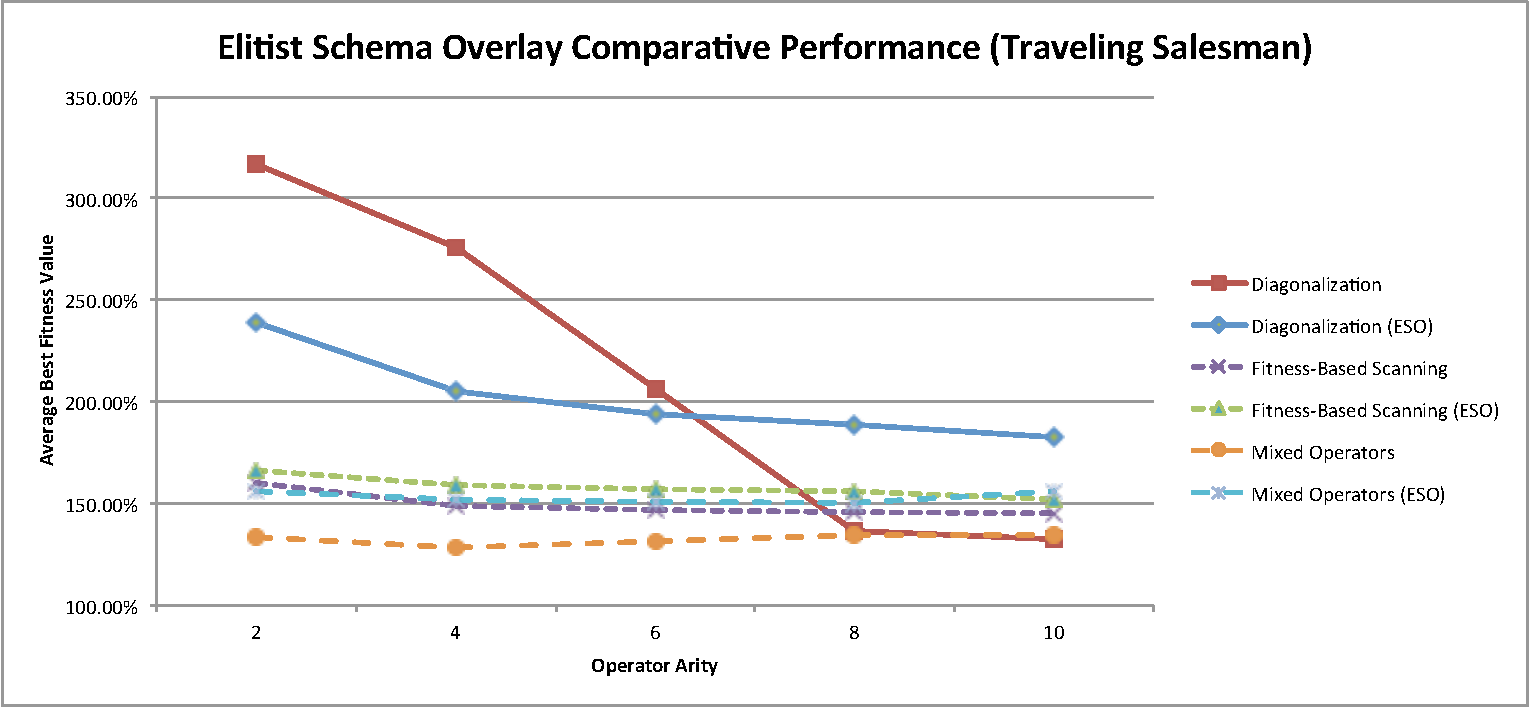
\includegraphics[scale=0.60]{charts/Both_TSP.pdf}
\caption{Comparative Performance on the Traveling Salesman Problem}
\label{fig:both_tsp}
\end{figure}

The Traveling Salesman Problem instances tested showed similar trends to the experiments with the Knapsack Problem (referenced in Figure \ref{fig:both_tsp}). When elitist schema overlays were used, the solutions found by traditional Genetic Algorithms were $78.03$ percentage points closer to the best found solution when averaged across all instances and problem sizes. Diagonalization with arity 4 also had significant gains when utilizing elitist schema overlays, with solutions improving on average by $70.75$ percentage points; however, on average performance dropped by $5.92$ percentage points.


NK-Landscape problem instances generated the same behavior as before, and elitist schema overlays consistently converged to the best found solution across all trials, regardless of which operator it was used in conjunction with. Thus, little more can be gained from examining that data. Now that we have finished analyzing the data concerning solution quality, we will examine how elitist schema overlays affect the runtime of Genetic Algorithms empirically. 

\begin{figure}[htbp!]
\centering
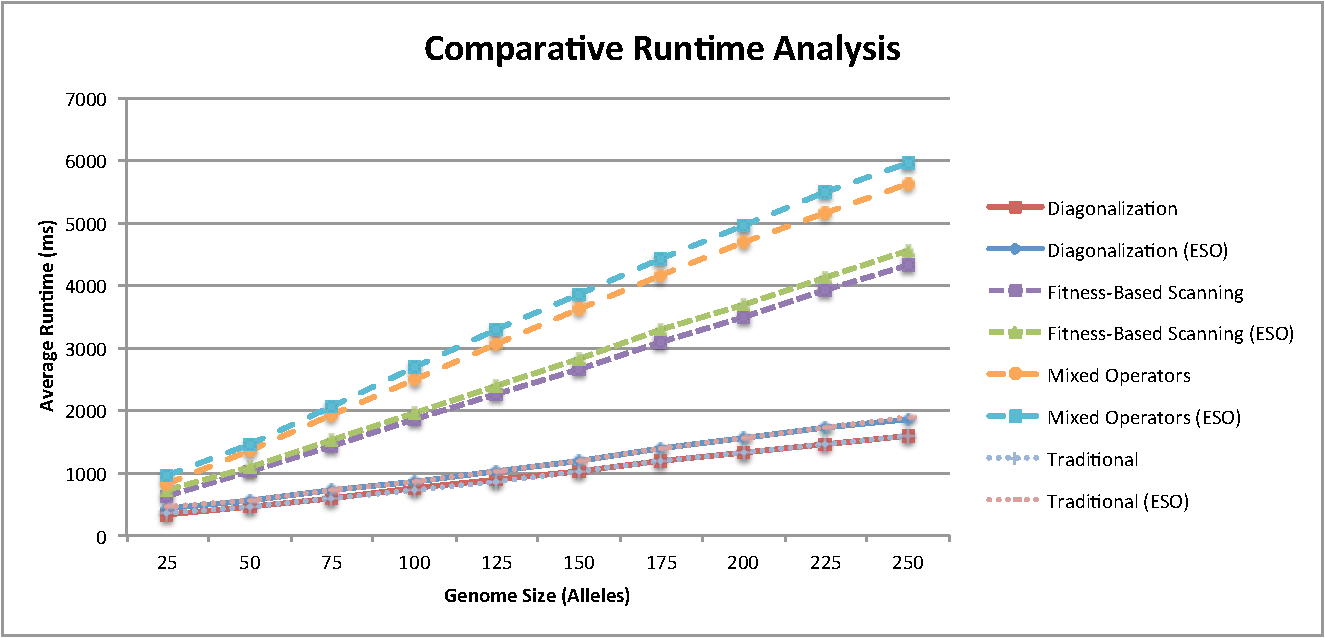
\includegraphics[scale=0.60]{charts/Runtime.pdf}
\caption{Comparative Runtime Analysis}
\label{fig:runtime}
\end{figure}

To determine if elitist schema overlays are prohibitively expensive in practice, we compared the runtimes of traditional Genetic Algorithms and multi-parent operators of arity $4$ both with and without elitist schema overlays on instances of increasing size of De Jong's Hypersphere Function (referenced in Figure \ref{fig:runtime}). Not only will this data illuminate the cost of utilizing elitist schema overlays, but it will also show how expensive traditional and multi-parent operators are in relation to each other. Traditional Genetic Algorithms ran the quickest in all instances, narrowly outperforming Diagonalization. Fitness-based scanning took significantly longer than both of these, and multi-operators naturally took longer still. In each instance, the addition of elitist schema overlays slowed genetic algorithms down, but only slightly. The whole of this data was used to derive our conclusions from our experiments.